\documentclass[12pt]{article}

\usepackage{sbc-template}
\usepackage[utf8]{inputenc}
\usepackage[brazil]{babel}
\usepackage{graphicx}
%\usepackage{booktabs}
\usepackage{amsmath}


\title{Visualização de Dados -- Trabalho Prático 1}

\author{Danilo Ferreira, Guilherme Avelino, Hudson Borges, Mauri Miguel}


\address{Departamento de Ciência da Computação, UFMG
%\email{\footnotesize \{danilofs,mtov\}@dcc.ufmg.br}
}


\begin{document}

\maketitle

%\section{Introdução}




\section{Abordagem Proposta}

TODO


\begin{figure}[h!]
  \caption{Visualização proposta}
  \centering
  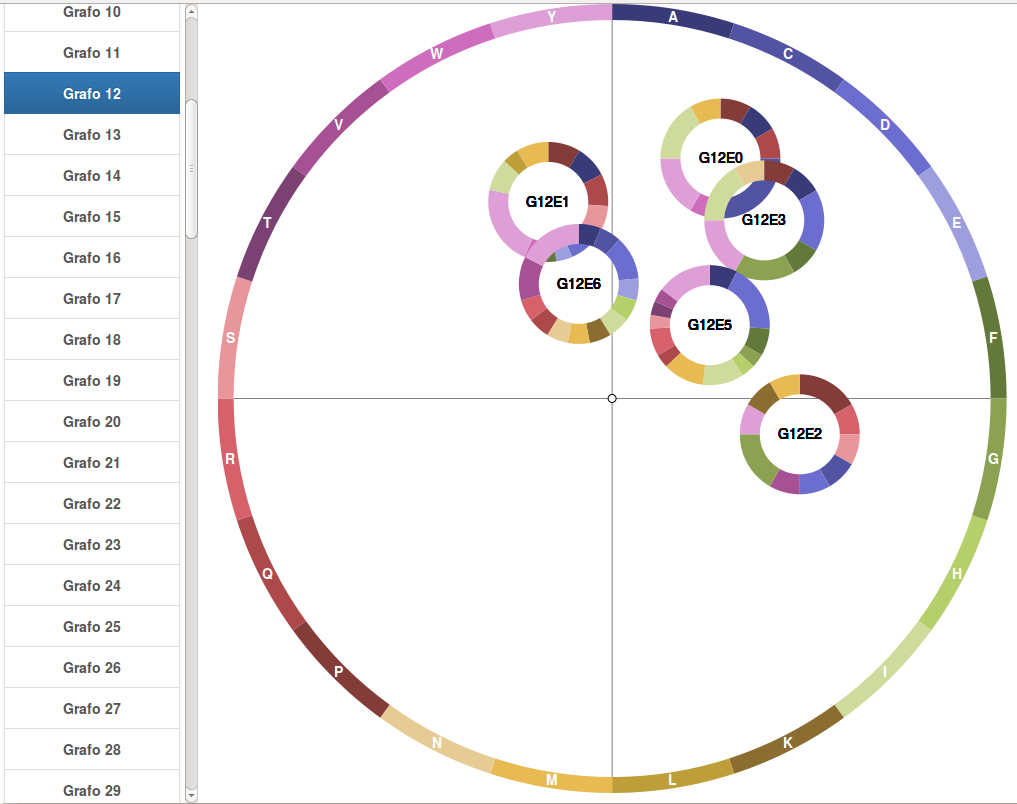
\includegraphics[width=0.8\textwidth]{visualizacao.png}
\end{figure}


\subsection{Cálculo da Similaridade}

Para calcular um índice de similaridade entre as pessoas, adotamos o modelo de espaço vetorial, a métrica TF-IDF ({\em Term Frequency - Inverse Document Frequency}) e a similaridade do cosseno, que são técnicas tradicionalmente utilizados em sistemas de recuperação de informação~\cite{manning2008}. Cada pessoa é representada como um vetor no espaço $n$-vetorial, onde cada dimensão representa uma categoria de local visitado. Seja $p \in P$ uma pessoa do conjunto $P$ de todas as pessoas e $c$ uma categoria de local. Cada componente do vetor é o produto entre os fatores $\text{tf}(c, p) \times \text{idf}(c, P)$, onde:
\begin{itemize}
\item $\text{tf}(c, p)$ é a frequência de visitas de $p$ a locais da categoria $c$.
\item $\text{idf}(c, P)$ é uma medida de quanta informação uma categoria $c$ fornece. Isto é, quanto mais comum é uma pessoa visitar uma categoria, menos representativa ela é para distinguir essa pessoa das demais. O componente $\text{idf}(c, P)$ é computado como:
\begin{align*}
\text{idf}(c, P) = \log \frac{|P|}{1 + |\{p \in P : \text{$p$ visita $c$}  \}|}
\end{align*}
\end{itemize}

Por fim, dados dois vetores $v$ e $u$ de componentes TF-IDF, a similaridade entre eles é calculada usando a similaridade do cosseno, que é definida como:
\begin{align*}
\text{sim}(v, u) = \frac{v \bullet u}{||v|| \times ||u||} = \frac{\sum_{i=1}^{n} v_i \times u_i}{\sqrt{\sum_{i=1}^{n} (v_i)^2} \times \sqrt{\sum_{i=1}^{n} (u_i)^2}}
\end{align*}




\section{Análise dos Dados e Descobertas}

\subsection{Lugares mais visitados}

Foi observado que grande parte dos grafos apresentou uma grande concentração de pessoas no primeiro quadrante (superior direito) da visualização proposta. Isso mostra que as pessoas de tais grafos possuem costumam vizitar mais frequentemente os lugares representados pelo primeiro quadrante. Por outro lado, o terceiro quadrante (inferior esquerdo) apresentou a menor concentração de visitas na grande maioria dos grafos, indicando que as pessoas de tais grafos visitam menos frequentemente, ou não visitam, os lugares representados por tal quadrante. Os quadrantes 2 e 4 apresentaram na maiorias dos grafos a mesma quantidade de visitação aos respectivos lugares, sendo a concentração de pessoas menor que a do primeiro quadrante e maior que a do terceiro quadrante.

\subsection{Costumes similares}

Como discutido na seção anterior, alguns subconjuntos de lugares (quadrantes) apresentam maior ou menor concentração de pessoas. Além disso, foi observado também que o posicionamento dessas pessoas dentro do mesmo quadrante são muito próximos e até mesmo sobrepostos em alguns momentos. Isso mostra que na maioria dos grafos as pessoas possuem costumes similares, no sentido que várias pessoas de um mesmo grafo visitam mais vezes os mesmos lugares.

\section{Conclusão}

TODO


\footnotesize
\bibliographystyle{abbrv}
\bibliography{tp1}

\end{document}
